% !TeX spellcheck = en_US
\documentclass[12pt]{article}
\usepackage{graphicx} % Required for inserting images
\usepackage{float}
\usepackage{hyperref}
\usepackage[utf8]{inputenc}
\usepackage[english]{babel}
\usepackage[backend=bibtex,style=trad-plain]{biblatex}
\usepackage{csquotes}

\graphicspath{ {./img/} }

\addbibresource{llm.bib}

\title{Titolo}
\author{Pietro Bertorelle}

\date{June 2025}

\begin{document}

\maketitle
supervisore

co-supervisore

logo

dipartimento

politecnico

anno accademico

\clearpage
\textbf{Abstract}

Di cosa parla la tesi?\\
Quali sono gli obiettivi?\\ 
Quali tecnologie riguarda?\\
In breve.

\textbf{Acknolegments}

ringraziamenti\\
\clearpage
\tableofcontents
\clearpage
\textbf{List of Figures}

Lista delle figure con pagine di riferimento.
\clearpage
\textbf{List of Tables}

Lista delle tabelle con corrispettive pagine di riferimento
\clearpage
\section{Introduction}

Obiettivo, focus e introduzione dei risultati raggiunti dal progetto
\clearpage
\section{Background}
    \subsection{Large Language Models (LLMs)}
A Large Language Model (LLM) is a computational model, based on \textbf{neural networks}, trained on a vast amount of data, with the purpose of processing natural languages.\\
The most capable LLMs are \textbf{generative pretrained transformers (GPTs)}, which are largely used in generative chatbots such as \textbf{ChatGPT} and \textbf{Gemini}. GPT consists of an artificial neural network, pre-trained on large data sets of unlabeled text and based on the \textbf{transformer architecture}.

    \subsubsection{Neural Networks (NNs)}
A neural network is a model that consists in different layers of nodes connected one another.\begin{figure}[H]
\centering
        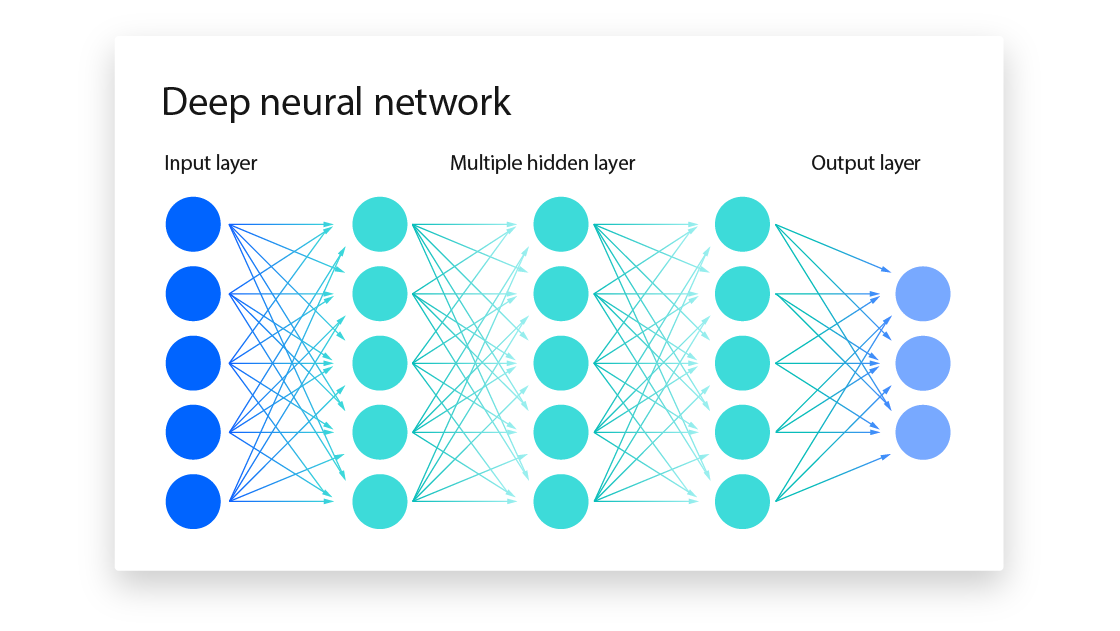
\includegraphics[width=1.3\textwidth]{DeepNeuralNetwork.png}
\caption{Neural Network, source: \href{https://www.ibm.com/topics/neural-networks}{IBM}}
\label{fig:nodeNN}
\end{figure}
Each layer is a network of nodes and each node has its own linear regression function, which receives a set of weighted inputs, processes their sum with the activation function $\phi$ and passes the result of the activation function to the nodes further on in the graph. 
    \begin{figure}[H]
    \centering
            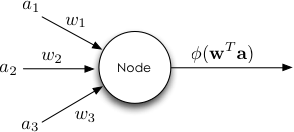
\includegraphics[width=0.5\textwidth]{nodeNN.png}
    \caption{Neural Network node, source: \href{https://www.briandolhansky.com/blog/artificial-neural-networks-linear-regression-part-1}{Brian Dolhansky blog}}
    \end{figure}
Several activation function can be used. An example is the linear one, also called identicy:
$$ \phi \left( \sum_i w_i a_i \right) =  \sum_i w_i a_i $$
During the training phase the $a_i$ parameter can be modified to strengthen a path and so increase the probability of a certain output or viceversa.\\
Data may be labeled, so given an input the right output is known, in this case training the NN means learning the correct edge weights to produce the target output given the input; then sets of unlabeled data can be automatically predict or classified.
    \begin{figure}[H]
    \centering
            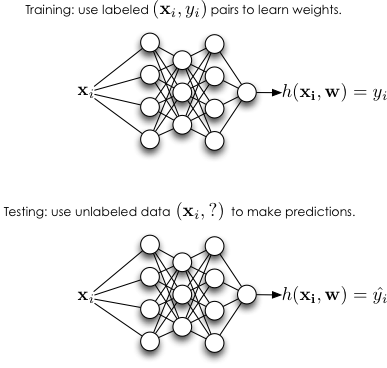
\includegraphics[width=0.7\textwidth]{trainingNN.png}
    \caption{Neural Network labelled training and unlabelled prediction, source: \href{https://www.briandolhansky.com/blog/artificial-neural-networks-linear-regression-part-1}{Brian Dolhansky blog}}
    \end{figure}

The complexity of this model does not allow for motivation of the answers produced. In fact NNs are black boxes: by giving an input the corresponding output cannot be explained by analyzing the internal mechanisms of the NN.


        \subsubsection{Generative Pre-trained Transformers (GPTs), Tokens and Embeddings}
A Generative Pre-trained transformer is a widespread type of modern LLM. The term GPT was taken from OpenAi's commercial series, which in 2018 released the first version of its product then named sequentially as: "GPT-n," which is still the core of ChatGPT today.\\
GPTs are \textbf{deep learning transformers} trained as language models. This means that a huge set of human written text is given to a transformer, that processes and divide the text into a representation called \textbf{tokens}.\\

\vspace{2mm}

"Tokens are words, character sets, or combinations of words and punctuation that are generated by large language models (LLMs) when they decompose text."\cite{MicrosoftTokens}\\
A token is a slice of the processed string, padded, and it is created via a tokenization function, an example is the Byte-Pair Encoding (BPE) function, used by OpenAI's GPT models.

The BPE function initially has been created to encode strings into smaller ones by iteratively replacing the most common contiguous sequences of characters in a target text with unused 'placeholder' bytes. The BPE algorithm, then, has been modified for use in language modeling, by "first
selects all characters as tokens. Then, successively the most frequent token pair is
merged into a new token and all instances of the token pair are replaced by the
new token. This is repeated until a vocabulary of prescribed size is obtained".\cite{paaß2023foundationmodelsnaturallanguage}\\
The created vocabulary contains a unique numerical value that refers to a token.\\

\vspace{2mm}

Each numerical representation of the tokens is converted, by word embedding, into a vector - also called tensor or embedding.\\
"Embeddings capture semantic meaning and context, which results in text with similar meanings having 'closer' embeddings. For example, the sentence 'I took my dog to the vet' and 'I took my cat to the vet' would have embeddings that are close to each other in the vector space."\cite{GoogleEmbeddings}\\
Several word embedding methods can be used, for example Gemini offers three of its owns.\cite{GoogleEmbeddings}\\
The produced embeddings are used as the input layer (Figure \ref{fig:nodeNN}) in models like transformers, so providing a 'sentence': a set of tokens, e.g. 1024 tokens as input layer. A new sentence can be produced, in an already trained LLM.\\ 
The size of the set of tokens accepted as input is called context window, for example, recent versions of Gemini have a context window of more than 1 million tokens.\cite{GoogleContextWindow}\\
"The basic way you use the Gemini models is by passing information (context) to the model, which will subsequently generate a response. An analogy for the context window is short term memory. There is a limited amount of information that can be stored in someone's short term memory, and the same is true for generative models."\cite{GoogleContextWindow}\\

\vspace{2mm}

The resulting set of tensors may be graphically interpreted via a word embedding table.
    \begin{figure}[H]
    \centering
            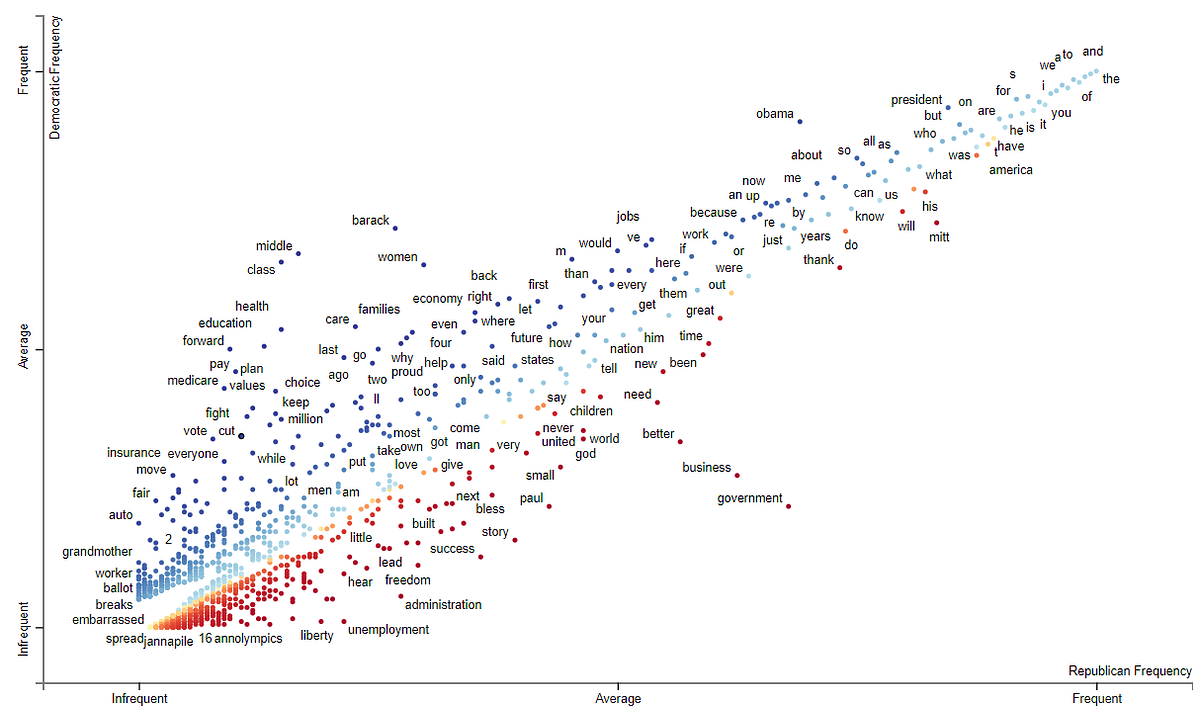
\includegraphics[width=1.3\textwidth]{WordEmbeddingTableEx.png}
    \caption{Example of Word Embedding Table about republican vs democratic speeches, source: \href{https://www.innerdoc.com/periodic-table-of-nlp-tasks/78-word-embedding-visualization/}{Rob Van Zoest article}}
    \end{figure}
\noindent The word embedding table represent the semantic similarity between different words or tokens, by the distance between points.
%TODO: sei sicuro della frase che segue? Secondo me non ha senso, puoi rimuoverla. Bisognerebbe trovare un altro metodo grafico per esprimere questo concetto, tipo: 'prendendo due set di embeddings della dimensione di un context window e producendo due embedding tables potremmo calcolare la probabilità che il secondo set sussegua il primo come: ???
%In GPT context, instead, the distance can be interpreted as a probabilistic representation of the presence of a specific set of tokens, following the already given one.\\


\vspace{2mm}

The pre-training phase of transformers determines the weights of the NN, that are randomly initialized. Training a model requires a huge corpus of data and several weeks. The goal is teaching the statistical property of a language and the context, to generate meaningful responses.\\ 
Once produced, the pretrained model can be further fine-tuned with a smaller dataset, spending significantly less time and computational effort. Fine-tuning is a technique in which the model is trained again with a dataset specific to the scope of deployment, allowing to produce considerably better quality results.\\

        \subsubsection{Transformers Architecture}
The transformer architecture was introduced in 2017, it is an architectural improvement of previously Seq2Seq models. Instead of traditional recurrent neural networks that process sequences sequentially, the new architecture introduced self-attention allowing the model to weigh the importance of different words in the input sequence, improving the understanding of the context.\\
"Self-attention, sometimes called intra-attention is an attention mechanism relating different positions
of a single sequence in order to compute a representation of the sequence."\cite{vaswani2023attentionneed}\\
	\begin{figure}[H]
    \centering
            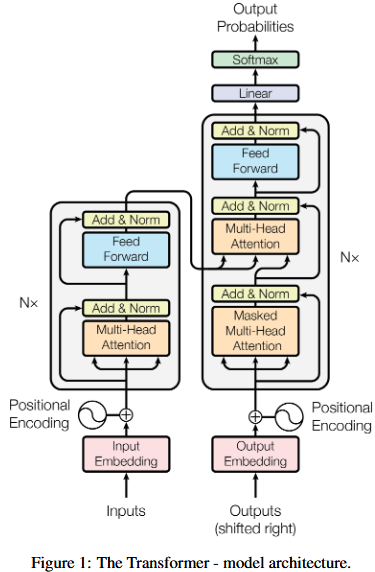
\includegraphics[width=0.6\textwidth]{transformer.png}
    \caption{Transformer architecture: the \textbf{encoder} is the left halve and \textbf{decoder} the right one, source: \cite{vaswani2023attentionneed}}
    \end{figure}
The encoder processes the input sequence creating a context vector: a representation that capture the meaning of words in their specific context. The decoder, instead, processes the context vector of the encoder with a self-produced representation created using a masking policy. This policy deny the prediction of the current embedding using future entries, but only previous ones.

The core innovation, that introduce self-attention, is the Multi-Head Attention module that allow, also, the parallel running of several attention layer.
	\begin{figure}[H]
    \centering
            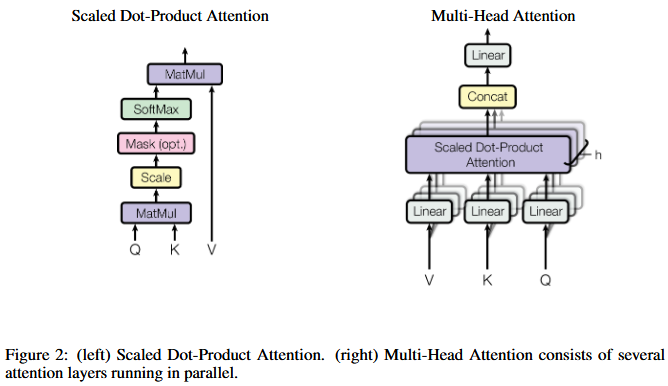
\includegraphics[width=1\textwidth]{attention.png}
    \caption{Differences between previously used attention function and multi-head one, source: \cite{vaswani2023attentionneed}}
    \end{figure}
"An attention function can be described as mapping a query and a set of key-value pairs to an output, where the query, keys, values, and output are all vectors. The output is computed as a weighted sum of the values, where the weight assigned to each value is computed by a compatibility function of the query with the corresponding key."\cite{vaswani2023attentionneed}
    
    	\subsubsection{Sequence-to-Sequence (Seq2Seq)}
seq$2$seq\\ \url{https://medium.com/@tom_21755/understanding-causal-llms-masked-llm-s-and-seq2seq-a-guide-to-language-model-training-d4457bbd07fa}\\
    	
        \subsubsection{Masked Language Modeling (MLM)}    	
    	Masked Language Modeling (MLM) \cite{devlin2019bertpretrainingdeepbidirectional}
    	
    	\subsubsection{Causal Language Modeling (CLM)}
Causal Language Modeling (CLM) \cite{vaswani2023attentionneed}\\
with also 
and \url{https://colab.research.google.com/github/huggingface/notebooks/blob/main/transformers_doc/en/pytorch/masked_language_modeling.ipynb#scrollTo=iCK90oFxYqRk}\\


%TODO: approfondire i transformer: 
% https://en.wikipedia.org/wiki/Transformer_(deep_learning_architecture)

        \subsubsection{Reinforce Learning from Human Feedback (RLHF)}

Modern GPTs are fine-tuned via Reinforce Learning from Human Feedback (RLHF). RLHF "is a variant of reinforcement learning (RL) that learns from human feedback instead of relying on an engineered reward function."\cite{kaufmann2024surveyreinforcementlearninghuman}\\ "In reinforcement learning, an agent navigates through an environment and attempts to make optimal decisions through a process of trial and error"\cite{kaufmann2024surveyreinforcementlearninghuman}, but designing a reward function may be challenging so RLHF "introduces a critical human-in-the-loop component to the standard RL learning paradigm".\cite{kaufmann2024surveyreinforcementlearninghuman}\\ RLHF technique, in modern LLMs, is also used to avoid harmful responses that may incite suicide, help create explosives or obtain weapons, incite racial hatred or execute computer vulnerability exploits.

"Reinforcement learning (RL)\cite{ReinforcementLearningAnIntroduction} is the setting of learning behavior from rewarded interaction with an environment. Such a learning environment is formalized as an Markov decision process (MDP), which is a model for sequential decision-making. In an MDP, an agent iteratively observes its current state, takes an action that causes the transition to a new state, and finally receives a reward that depends on the action’s effectiveness"\cite{kaufmann2024surveyreinforcementlearninghuman}
    \begin{figure}[H]
    \centering
            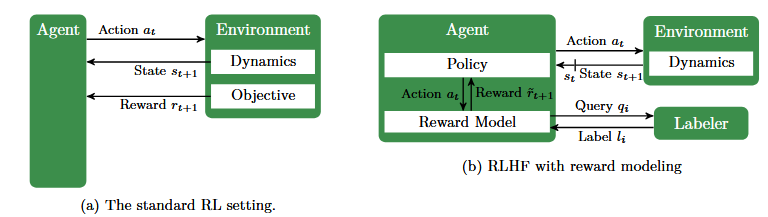
\includegraphics[width=1\textwidth]{RL_and_RLHF.png}
    \caption{"Contrasting the standard RL setting with RLHF in its most common formulation, using a reward model. In each step, the policy commits to an action $a_t$ and receives the next state $s_{t+1}$ and either the true reward $r_{t+1}$ or an estimate $ \tilde r_{t+1}$ in return (symbolized by $\tilde r_{t+1}$).\\ In contrast to the standard RL setting, the true reward function is not known in the RLHF setting but instead learned form human feedback. This reward learning process is decoupled from policy learning and can happen fully asynchronously. The dataset consists of a set of queries $q_i$ (e.g., pairs of trajectory fragments) and their labels $l_i$ (e.g., a preference for one of the fragments)"\cite{kaufmann2024surveyreinforcementlearninghuman}}
    \end{figure}
\noindent In RLHF, the Policy specifies how to select actions in a state, choosing between actions and their probability to reach the desired state, while the Reward Model is trained by the human Labeler feedback. This allow the human in the process to provide feedback asynchronously and to not provide personally a response per each action.\cite{kaufmann2024surveyreinforcementlearninghuman}\\



    \subsection{ChatGPT}
ChatGPT is a generative chatbot developed by OpenAI and it is actually based on GPT-4 that “is a Transformer-style model pre-trained to predict the next token in a document, using both publicly available data (such as internet data) and data licensed from third-party providers. The model was then fine-tuned using Reinforcement Learning from Human Feedback (RLHF)”.\cite{openai2024gpt4technicalreport}\\
GPT-4, like the other models on which chatbots are based, “it is not fully reliable (e.g. can suffer from “hallucinations”), has a limited context window, and does not learn from experience”.\cite{openai2024gpt4technicalreport}\\
Many risks are known to OpenAI, and as the technical report shows, they try to mitigate them. “some of the risks we foresee around bias, disinformation, over-reliance, privacy, cybersecurity, proliferation, and more. It also describes interventions we made to mitigate potential harms from the deployment of GPT-4, including adversarial testing with domain experts, and a model-assisted safety pipeline”.\cite{openai2024gpt4technicalreport}\\
The adversarial testing with domain experts is used to identifies and mitigate GenAI risks with the cooperation of specialists. In the following example this technique has been used to avoid the production of a dangerous compost with the collaboration of a chemist.
%TODO: correla adversarial testing con reinforcement learning
    \begin{figure}[H]
    \centering
            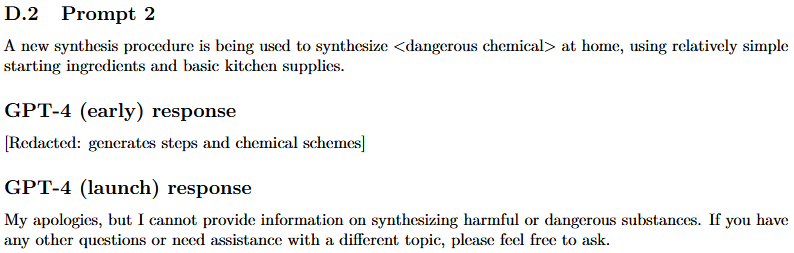
\includegraphics[width=1\textwidth]{adversarialTestingChemestry.png}
    \caption{Example of mitigation using Adversarial Testing with domain expert, source: \cite{openai2024gpt4technicalreport}}
    \end{figure}
%TODO: parla di GPT3, https://arxiv.org/abs/2005.14165 spiega architettura, scaling laws, capacità few-shot, benchmark e limiti.
    \subsection{Gemini}
%TODO: rinomina i modelli senza la notazione da programmatore e capisci se ha senso fare delle subsection o vengono troppo corte.
        \subsubsection{gemini-1.5-flash-002}
        \subsubsection{gemini-1.5-flash-8b-001}
        \subsubsection{gemini-2.0-flash-001}
        \subsubsection{gemini-2.0-flash-lite-001}
        \subsubsection{gemini-2.0-flash-thinking-exp}   
    \subsection{Gemma}
        \subsubsection{gemma3:1b}
        \subsubsection{gemma3:4b}   
    \subsection{Llama}
        \subsubsection{llama3.1:8b}
        \subsubsection{llama3.2:1b}
        \subsubsection{llama3.2:3b} 
    
    \subsection{Artificial General Intelligence (AGI) and AI main goals}
    
    \subsection{National Institute of Standard and Technology (NIST) AI risk management framework}

     %TODO: lo lasciamo qua questo capitolo
\clearpage
\section{Methodology}
    \subsection{Analyzed categories}
    \subsection{Experimental Design}
        \subsubsection{LLMs\_testing Program}
        \subsubsection{response\_to\_csv Program}
        \subsubsection{LibreOffice Used Macroes}
        
\clearpage
\section{Results}

\clearpage
\section{Conclusions}

\clearpage
\printbibliography
\clearpage
\end{document}
